\documentclass[12pt,letterpaper]{article}
\usepackage[utf8]{inputenc}
\usepackage{amsmath}
\usepackage{amsfonts}
\usepackage{amssymb}
\usepackage{graphicx}
\graphicspath{ {figures/} }
\usepackage{array}
\usepackage{caption}
\usepackage{float}
\usepackage{todonotes}
\usepackage{appendix}
\usepackage[backend=biber, style=numeric, citestyle=numeric]{biblatex}
\usepackage{tabularx}
\usepackage[margin=1in]{geometry} 
\usepackage{textcomp} %textdegree
\usepackage[space]{grffile} %permits space in includegraphics
%\usepackage{lipsum}
\usepackage{pgfplots}
\pgfplotsset{width=10cm,compat=1.9}
%%%%%%%%%%%%%%%%%%%%%%%%%%%%%%%%%%%%%%%%%%%%%%%%%%%%%%%%%%%% Preamble
% \addbibresource{flash biblio.bib}

\renewcommand{\listfigurename}{Figures}
\renewcommand{\listtablename}{Tables}
%\setcounter{secnumdepth}{0}
\setcounter{tocdepth}{2}
\setlength{\parindent}{0pt}
\setlength{\parskip}{1em}
\rmfamily

\author{Edvin Alvarado}
\title{Establishing a Progressive Income Tax System that Minimizes Disincentivization}
%%%%%%%%%%%%%%%%%%%%%%%%%%%%%%%%%%%%%%%%%%%%%%%%%%%%%%%%%%%% Document
\begin{document}
	
	% \begin{titlepage}
	% 	\centering
	% 	\large
	% 	University of Puerto Rico\\
	% 	Mayag\"uez Campus\\
	% 	Department of Chemical Engineering
		
	% 	\vfill
	% 	{\LARGE
	% 	\textbf{Establishing a Progressive Income Tax System that Minimizes Disincentivization}
	% 	}
	% 	\vfill
		
	% 	Prof. Glberto Villafa\~ne\\
	% 	INQU 5030-020\\
	% 	Experiment start date: December 20, 2017\\
	% 	Experiment end date:  December 20, 2017\\
	% 	Report submission date: January 3rd, 2018
		
	% 	\vspace{1cm}
		
	% 	Group 2\\		
	% 	Daiza P. M\'endez \\
	% 	Jennyliam Rodr\'iguez\\
	% 	Edvin Alvarado	(leader)	\\
	% 	Jean De Armas
	% \end{titlepage}
	\maketitle
	
	% \pagenumbering{gobble}
	% \tableofcontents	
	% \begingroup
	% \let\clearpage\relax %lets you join both lists somehow
	% \listoffigures	
	% \listoftables
	% \endgroup
	% %\clearpage
		
	\pagenumbering{arabic}
	\section{Incentivization} 
	
		As long as the Marginal Utility (UM) is greater than the Price (P) then it's worth getting more of that good. If UM is less than the Price, it is worse to consume one more. In a free competitive market, the Price will be equal to the Marginal Cost (CM). Therefore:

		\begin{align*}
			UM&>P \\
			UM-P&>0 \\
			UM-CM&>0
		\end{align*}

		The Net Marginal Utility (UMN) is the difference between UM and CM.

		\begin{align*}
			&UMN \equiv UM-CM \\
			&UMN > 0
		\end{align*}

		The UM and CM are the Derivatives of Total Utility (U) and Cost (C) respectively.

		\begin{align*}
			&UM \equiv \frac{\mathrm{d}U}{\mathrm{d}Q} \\
			&CM \equiv \frac{\mathrm{d}C}{\mathrm{d}Q} \\
			&UMN = \frac{\mathrm{d}U}{\mathrm{d}Q} - \frac{\mathrm{d}C}{\mathrm{d}Q}
		\end{align*}

		\section{The Marginal Utility of Money}

		The utility will always have decreasing marginal utility. The utility can always increase or reach a maximum point. In the case of money, I assume that more money always is better but the next dollar gives less utility than the former dollar. However, the next dollar would would never drop to negative utility. So the General Utility Function:

		\begin{equation}
			U(Q) = u_1 Q^{u_2}, \quad 0<u_2,<1
		\end{equation}

		% \begin{tikzpicture}
		% 	\begin{axis}
		% 		\addplot[color=red]{exp(x)};	
		% 	\end{axis}
		% \end{tikzpicture}

		\begin{tikzpicture}
		\begin{axis}[
		    axis lines = left,
		    xlabel = $Q$,
		    ylabel = {$U$},
		]

		\addplot [
		    domain=0:200000, 
		    samples=1000, 
		    color=red,
		]
		{1000*x^0.4};
		\addlegendentry{$U = 1000\ Q^{0.4}$}

		\addplot[
			domain=0:200000, 
		    samples=1000, 
		    color=black
		]
		{x};
		\addlegendentry{Q}

		\end{axis}
		\end{tikzpicture}
		%%%%%%% https://www.sharelatex.com/learn/Pgfplots_package

		It would not make much sense that a dollar would be worth less of a dollar. However, it is part of the limits of Microeconomics to value everything with money so we would just need to accept this. If this doesn't convince then I'll provide some decentish example. If we were to take 10\% of poor man and a rich man, the negative effects are vastly different. The poor man will have it worse even if the tax is equally proportional. The poor man might not be capable of making car payment, not pay some utilities, not making rent, making it hard to feed your family. While the rich man, might no be capable of getting a third car, a summer home, or that extra butler. It is obvious that the the poor man will suffer more than the rich man. This proves that proportional costs (flat taxes) don't equally distribute the utility costs of taxation. Only a progressive tax could achieve this by having the UMN to be roughly constant throughout all type of incomes.

		\section{Progressive Tax System}

		The cost of taxation is a percentage of gross income. Let T be the tax percentage:

		\begin{equation}
			C = T \times U
		\end{equation}

		Various progressive taxes with NIT were tried and the following model was established:


		\begin{equation}
			T = \begin{bmatrix}
				a \ln x-b, \quad x \leq \exp(\frac{t_m+b}{a}) \\
				t_m, \quad x \geq \exp(\frac{t_m+b}{a})
			\end{bmatrix}
		\end{equation}

		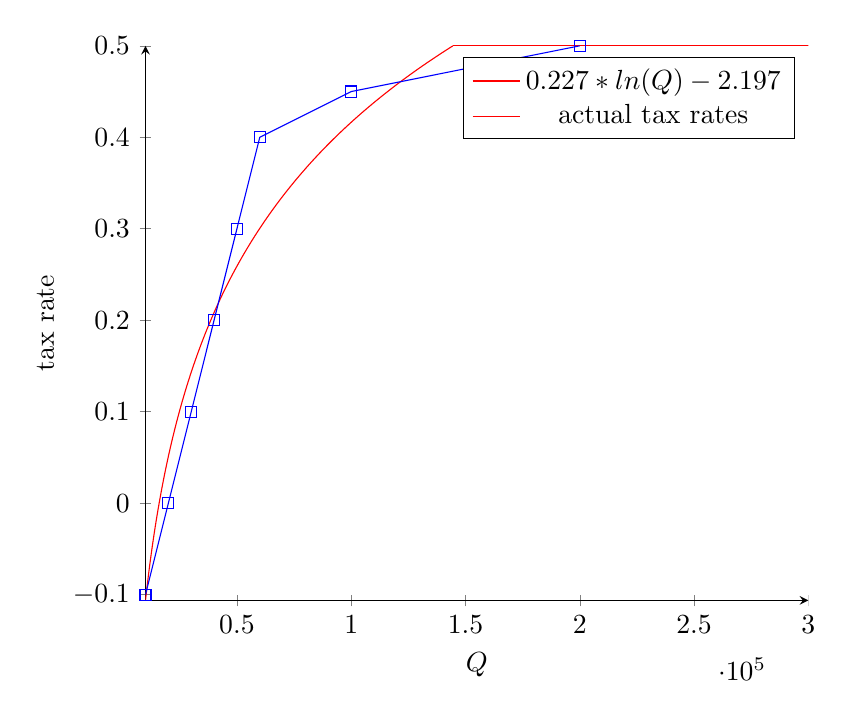
\begin{tikzpicture}
		\begin{axis}[
		    axis lines = left,
		    xlabel = $Q$,
		    ylabel = {tax rate},
		]

		\addplot [
		    domain=10000:144503, 
		    samples=1000, 
		    color=red,
		]
		{0.227 * ln(x)-2.197};
		\addlegendentry{$0.227 * ln(Q)-2.197$}

		\addplot[
			domain=144503:300000, 
		    samples=1000, 
		    color=red
		]
		{0.5};

		\addplot[
		    color=blue,
		    mark=square,
		    ]
		    coordinates {
		    (10000,-0.1)(20000,0)(30000,0.1)(40000,0.2)(50000,0.3)(60000,0.4)(100000,0.45)(200000,0.5)
	    };
	    \addlegendentry{actual tax rates}

		\end{axis}
		\end{tikzpicture}

		Where $t_m$ is the maximum tax rate. Although in real case the tax are based on brackets, a continuous tax rate was chosen to simplify calculations.

		\section{Establishing Net Marginal Utility}

			As all the equations and assumptions are set and explained, let's derive the the Net Marginal Utility.

			\begin{equation}
				UM = \frac{\mathrm{d}U}{\mathrm{d}Q} = u_1 u_2 Q^{u_2-1}
			\end{equation}
			I won't write the ranges to save time but they're all the same as the one stated in the previous sections.
			\begin{align}
				C = T*U = \begin{bmatrix}
					u_1 Q^{u_2} (a \ln Q - b) \\
					t_m u_1 Q^{u_2} 
				\end{bmatrix} \\
				CM =\frac{\mathrm{d}C}{\mathrm{d}Q} = \begin{bmatrix}
					u_1 Q^{u_2-1} \left[ a + u_2 (a \ln Q - b) \right] \\
					t_m u_1 u_2 Q^{u_2-1}
				\end{bmatrix}
			\end{align}

			\begin{equation}
				UMN = UM-CM = \begin{bmatrix}
					- \frac{u_1}{u_2} Q^{u_2 - 1} \left( a \ln Q + \frac{a}{u_2} - b - 1 \right) \\
					t_m u_1 u_2 Q^{u_2-1}
				\end{bmatrix}
			\end{equation}

			Because I'm lazy, instead of modeling these in \LaTeX with pgfplots I'll take a screen shot of the Geogebra document used.
		
			\begin{figure}[H]
				\centering
				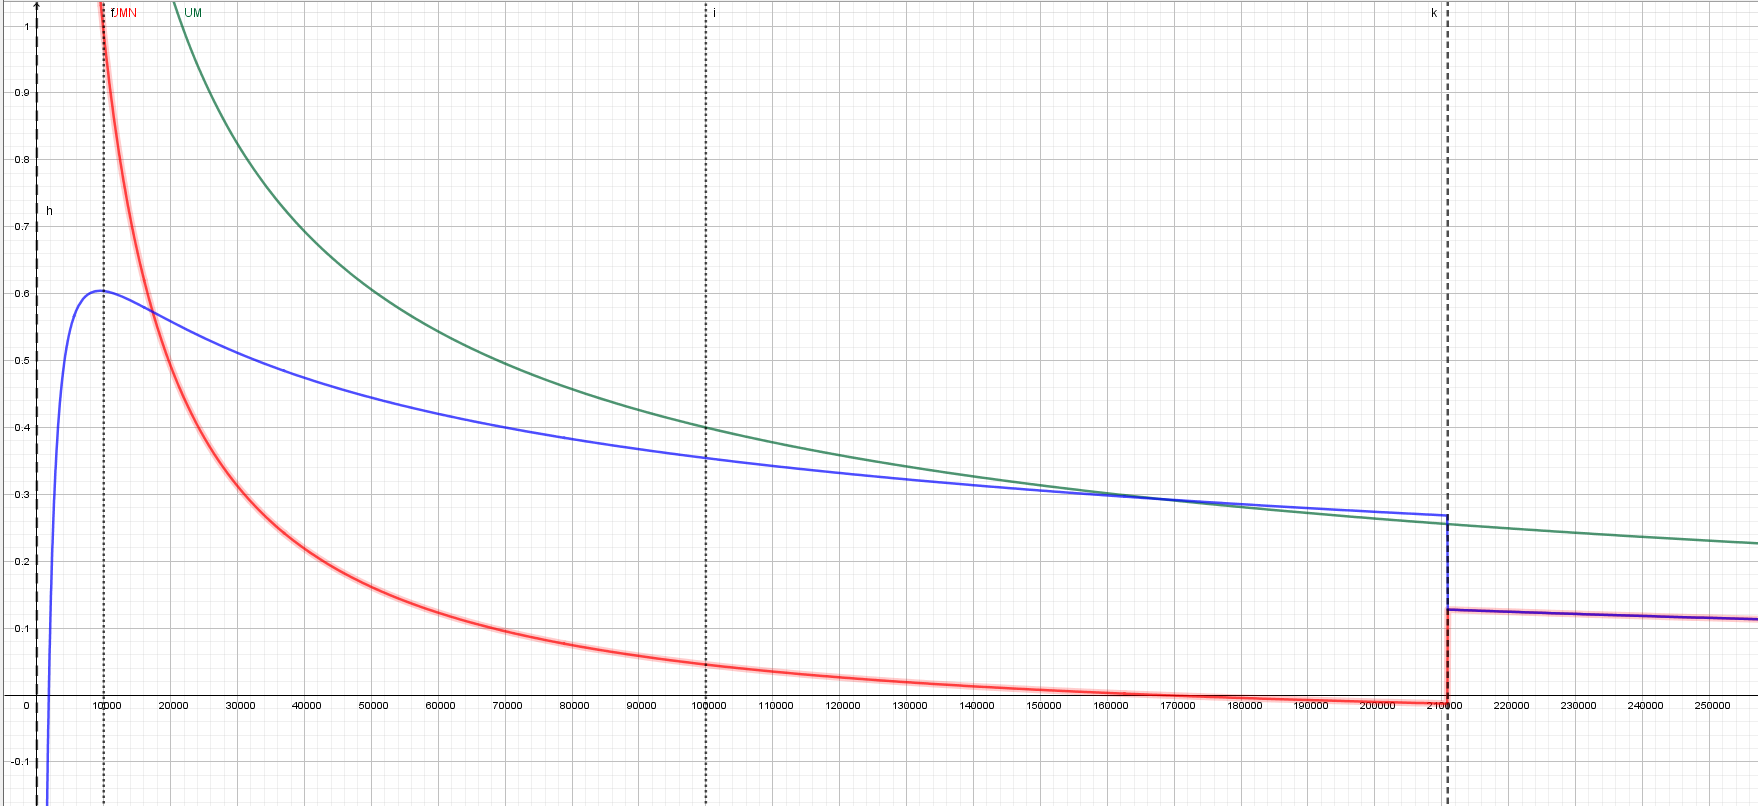
\includegraphics[width=\textwidth]{graph}
				% \caption{Caption here}
				\label{fig:figure1}
			\end{figure}

			Notice that then UMN does go under zero, meaning that those with income in the range of negative UMN will be better off not gaining another dollar. This is problematic, so this should be eliminated if possible. UMN is negative from a point $Q_i$ to $Q_m$, where $Q_m = \exp(\frac{t_m+b}{a})$.

			\begin{align*}
				UMN(Q \neq 0) = 0 = a \ln Q_i + \frac{a}{u_2} -b -1 \\
				Q_i = \exp \left(\frac{b-1}{a}- \frac{1}{u_2}\right)
			\end{align*}

			% \begin{tikzpicture}
			% \begin{axis}[
			%     axis lines = left,
			%     xlabel = $x$,
			%     ylabel = {$y$},
			% ]

			% \addplot [
			%     domain=-5:5, 
			%     samples=100, 
			%     color=red,
			% ]
			% {exp(x)};
			% \addlegendentry{$e^x$}

			% \end{axis}
			% \end{tikzpicture}

			All the variables were manipulated and it is impossible to eliminate this negative UMN area. At least without changing the General Utility Equation and eliminating progressive tax. Therefore the goal should be to minimize it as much as possible:

			\begin{equation}
				\int^{Q_m}_{Q_i} UMN \ dQ = 0^-
			\end{equation}

			\begin{equation}
				\int UMN \ dQ = - \frac{u_1}{u_2^2} Q^{u_2} (a \ln Q -b-1)
			\end{equation}

			The variables $a, b, t_m, u_1, u_2 $ were manipulated. However, the focus was on manipulating $t_m$ to minimize the Negative UMN Area. Overall, The observations showed that a top tax rate of over 50\% increases this area considerably. that the top tax rate that minimizes the area was 43-45\%.
		
	%\cite{main}
	% \nocite{*}
	% \printbibliography
	%\clearpage
	
%	\appendix
%	\chapter{aaa}
%	\section{bbb}
	
\end{document}

